\chapter{数据交换子系统的详细设计与实现}
\section{仿真机侧数据交换模块}
仿真机侧数据交换模块负责虚拟仿真机与仿真机之间的交流。仿真机侧发送出的数据帧仅被以太网协议封装过,即除去数据内容外,仅含有以太网协议头。
此种数据帧如果交给虚拟仿真机的网络协议栈处理将不能得到正确内容。因此在实现中虚拟仿真机需要绕过网络协议栈直接接手数据帧自行处理。
该模块会将收到的数据帧解封,并拆解为多条仿真机指令供后续使用,或者将多个仿真机反馈指令粘合,并自行添加以太网协议内容封装为数据帧发送给仿真机。
\subsection{流程图}
\par
本模块的主要执行流程如图\ref{module11}所示。流程分为接收消息和发送反馈消息两部分。虚拟仿真机在接收到原始数据帧后首先取得头部中的指令部分总长度信息,跳过头部后,根据每条指令的长度信息将粘合在一起的多条指令进行拆分,交付给转换模块。
当总长度读取完毕后,数据帧的接收流程便结束。此过程中可能遇到暂时没有验证的仿真机指令,将其暂时丢弃即可。
\par
反馈消息流程中,该模块会收到来自指令转换模块的仿真机指令,其需要将这些指令粘合并为它们添加总长度、以太网协议头等信息构建成一个数据帧,最后将其写入发送队列结束流程。
\clearpage
\begin{figure}[h!]
    \begin{center}
        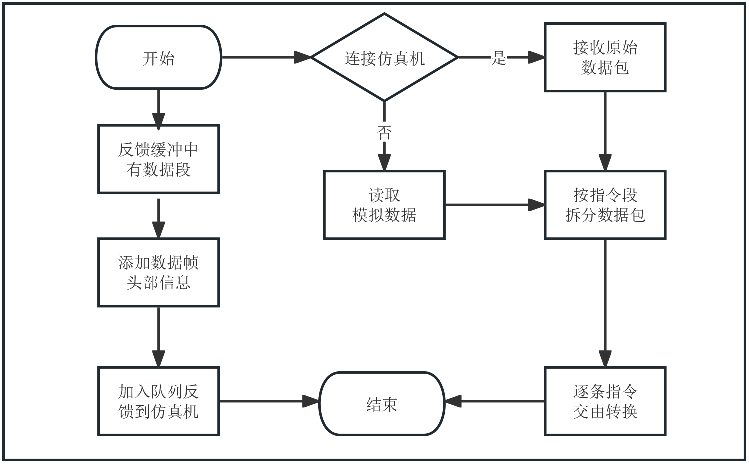
\includegraphics[width=0.8\textwidth]{pictures/flowchart1.pdf}
        \caption{仿真机侧数据交互流程图}
        \label{module11}
    \end{center}
\end{figure}
\subsection{核心类图}
\par
本模块的核心类图如图\ref{module12}所示。其中的核心是类SimulationDeviceContext,它表示仿真机与虚拟仿真机的交流环境
MacLinkCommunication类负责初始化与某一网卡设备的侦听关系,并负责数据帧的实际收取和发送。
MacReceivingRunnable是处理信息收发的线程实例,收取到的数据帧会加入接收数据帧的队列MacReceivingQueue,线程实例从中取数据并交由指令转换模块。
当需要反馈时,线程实例会调用设备实例中的发送方法,最终通过MacLink实现发送。
ISimulatorDeviceInterface代表仿真机设备类的接口,其中包含了对于数据帧中指令代号的读取方法GetSimOperateCode,以及发送消息给仿真机SendToSimulationDevice方法。
CAEGenericSimulatorDeviceBase是该接口的一个实现,其代表CAE公司的仿真机设备,其中含有解读并转换该设备指令的具体算法。当需要接入其他公司设备时,
只需要重新实现SimulatorDevice接口。
\clearpage
\begin{figure}[h!]
    \begin{center}
        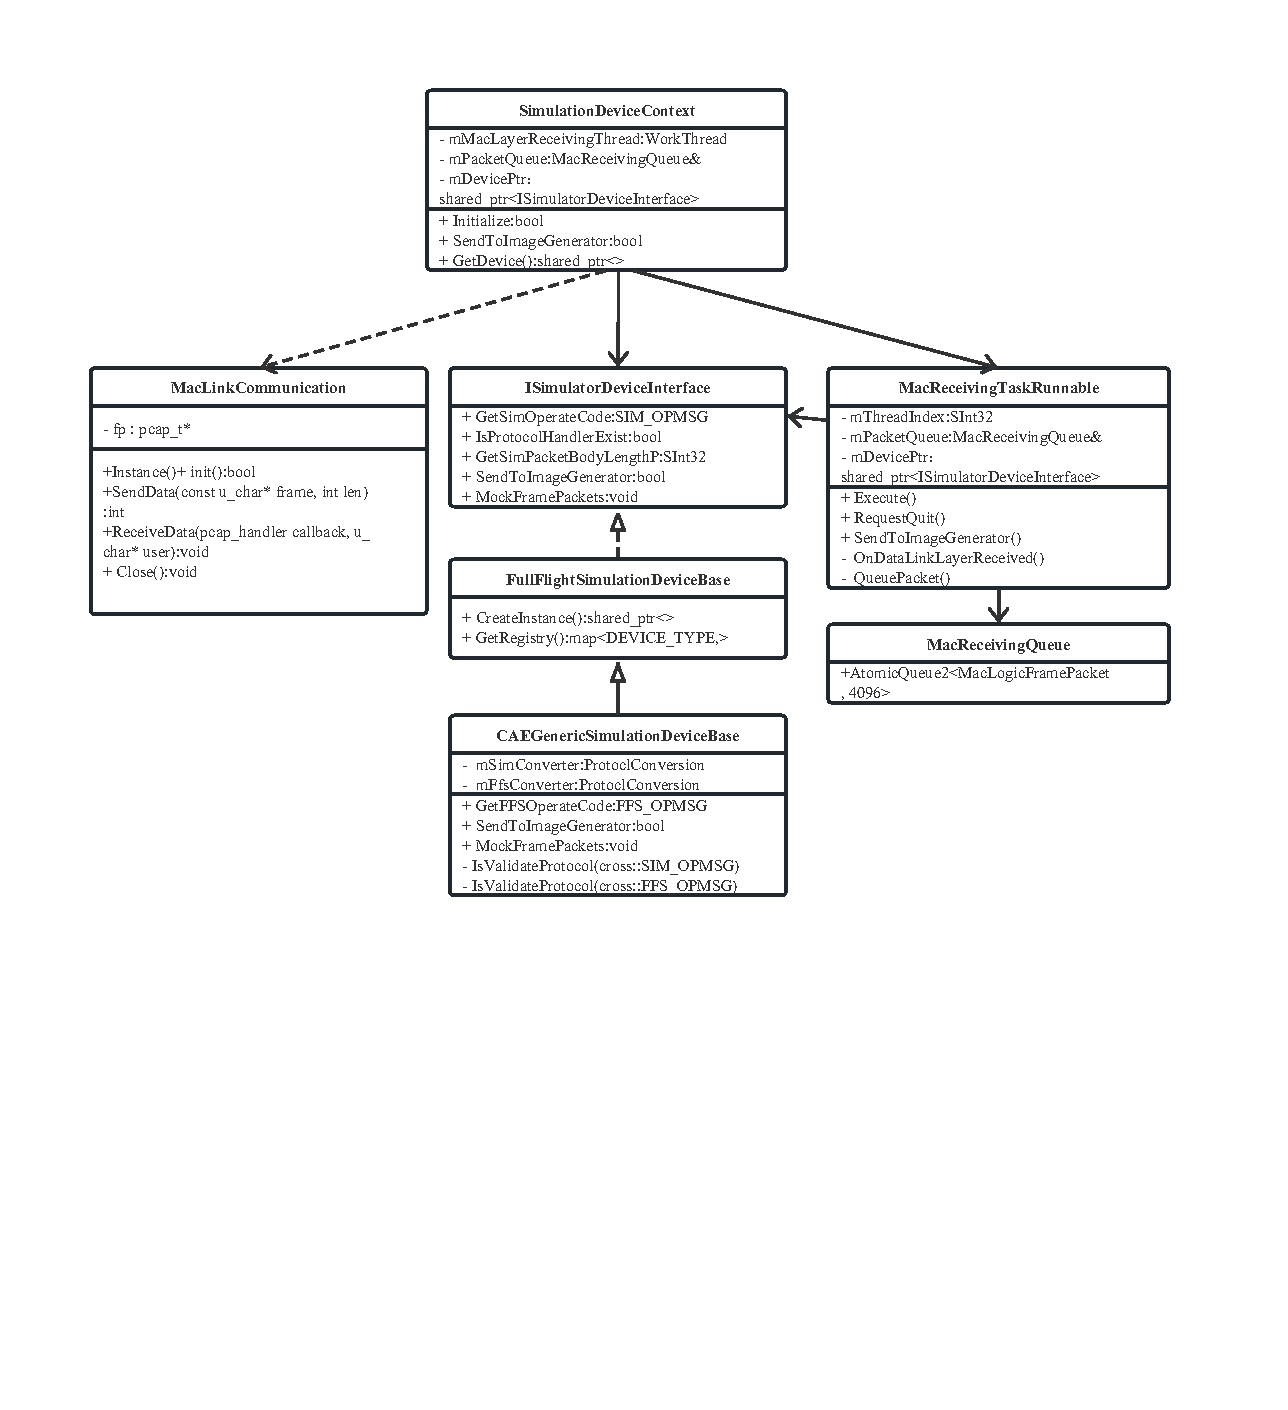
\includegraphics[width=\textwidth]{pictures/classdiagram1.pdf}
        \caption{仿真机侧数据交互核心类图}
        \label{module12}
    \end{center}
\end{figure}
\subsection{顺序图}
图\ref{seq1}是仿真机侧数据交换模块的顺序图,描述了仿真机与虚拟仿真机沟通过程中各类的交互过程。
首先交流环境类SimDeviceContext以mac地址作为参数尝试初始化MacLink,即开始侦听对应网卡设备,MacLink类中利用WinpPcap实现侦听,并判断是否侦听成功。
成功建立连接后,便可以进行数据的收发。交流环境线程MacTaskRunnable运行后会循环执行OnMacRecevied方法,
当有数据到达时会对其进行解封处理并加入MacQueue队列等待指令转换。
当有消息需要反馈时,交流环境调用线程实例的send方法,线程实例调用具体设备实例的send方法,而设备实例最终通过MacLink对象实现发送。
\begin{figure}[h!]
    \begin{center}
        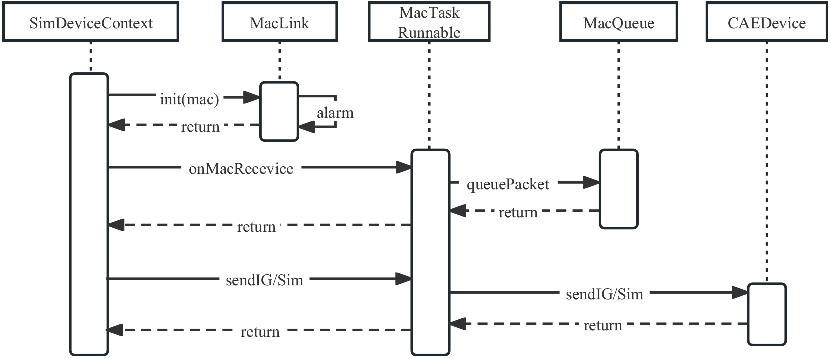
\includegraphics[width=\textwidth]{pictures/sequence1.pdf}
        \caption{仿真机侧数据交换顺序图}
        \label{seq1}
    \end{center}
\end{figure}
\subsection{关键代码}
图\ref{codeSimRec}中是虚拟仿真机接收数据帧时的代码。当有数据包达到时,OnDataLinkLayerReceviced会作为回调函数被被调用。
参数pkt\_data是收取到的数据流指针,类型为u\_char*表示要按字节读取数据流中的信息。outPackets是该方法的输出结果,一个数据帧中可能含有多条仿真机指令,这些指令所在的数据段被拆分后放入集合outPackets中。
\par
临时变量cursor指向数据流中当前正被处理的字节,其初始指向位置与pkt\_data相同。
首先应该跳过数据帧的头部,如第三章第一节中提到的数据帧组织结构,数据帧头部含有以太网协议头、CAE头等信息,通过ParseMacLinkLayerHeader方法保留这部分头部信息,同时跳过对应的长度,使指针cursor来到数据帧中的指令部分。
\par
数据帧头部信息中含有该帧除去头部的长度,使用临时变量leftBytesToRead保存。当其仍大于零时,说明还有仿真机指令没有读取。
每条指令的头部特定位置也有单一指令的长度,是以4字节为单位,curPacketLength计算了该指令以字节为单位的长度。有了这些信息,便能够以cursor为起点,curPacketLength为长度拷贝指令段到一个packet中。
这样就完成了一个仿真机指令的拆分,当读取完整个数据帧后,虚拟仿真机便完成了接收数据帧的过程。
\begin{figure}[h!]
    \centering
     \lstinputlisting[basicstyle= \zihao{-5}]{pictures/SimReceive.txt}
    \caption{接收数据帧代码}
    \label{codeSimRec}
\end{figure}
\par
来自图像生成器的反馈信息最终也会以数据帧的形式给到仿真机。该方法的参数就是一组待发送仿真机指令的引用,
每个指令中含有自己的指令代号opCode和指令长度packetLength。首先需要将全部的仿真机指令粘合在一起,存储在generator\_body中。
期间需要对指令长度长度进行累积计算,totalPacketLength作为最后整个数据帧头部的长度信息。
\clearpage
\par
完成仿真机指令的粘和后,便需要根据规则构建一个可供仿真机使用的数据帧。首先是添加以太网协议头、CAE头等头部信息。其次将粘合后的指令集generator\_body添加在头部信息后。
最后还需要添加一个4字节的全为0的尾部,一个数据帧便构建完成。此数据帧不需要任何数据交换协议的变化,直接以原始二进制的形式通过WinPcap最终发出。
\begin{figure}[h!]
    \centering
     \lstinputlisting[basicstyle= \zihao{-5}]{pictures/SimSend.txt}
    \caption{发送数据帧代码}
    \label{codeSimSend}
\end{figure}

\section{指令转换模块}
指令转换模块负责仿真机指令与自定义指令之间的转换。经过转换后的指令才能被对方理解并使用。首先仿真机指令中对于浮点数的表达方式是由该厂商自行设计的,对于不同用途不同精度要求的数据其数字表示方式均存在差异。
因此这两种结构之间的转换需要严格依照设计文档中的说明设计转换算法,而不是简单的赋值。
其次仿真机指令中最重要的无疑是关于飞机位置和姿态的指令,但由仿真机给出的位置是由经纬度高度组成的数据,而图像生成器中使用的坐标系是笛卡尔坐标系,必须经过坐标系的转换才能使用该信息。
\subsection{流程图}
\par
本模块的主要执行流程如图\ref{module21}所示。
当收到来自仿真机的指令段时,数据转换模块先根据指令代号确定指令类型,用对应的仿真机指令结构体实现反序列化,再根据指令代号查找出对应的转换器,该转换器中的转换方法可将该指令转换为对应的自定义指令。
当收到自定义指令时,同样根据指令类型查找相应的转换器,使用该转换器中的方法完成转换。
\begin{figure}[h!]
    \begin{center}
        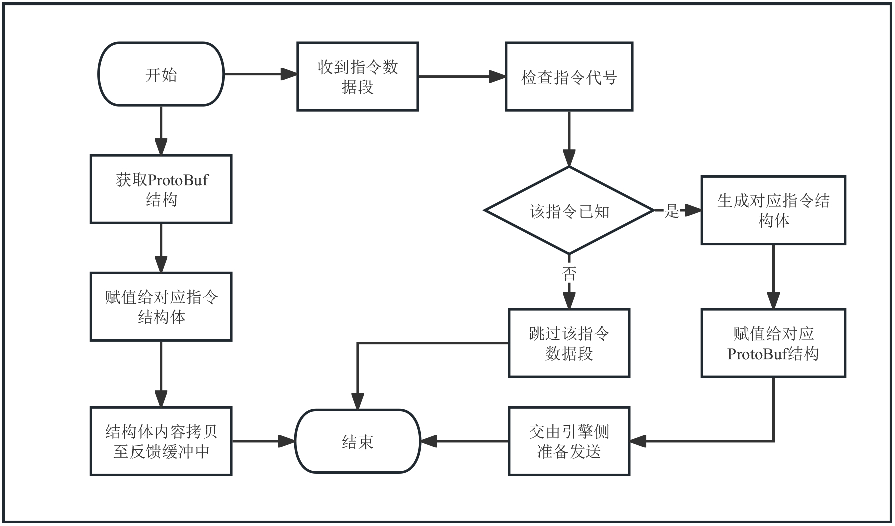
\includegraphics[width=0.8\textwidth]{pictures/flowchart2.pdf}
        \caption{数据转换流程图}
        \label{module21}
    \end{center}
\end{figure}
\subsection{核心类图}
\par
本模块的核心类图如图\ref{module22}所示。其中核心为IProtoclConversion接口,该接口中声明了仿真机指令与自定义指令间转换的方法Convert。需要注意的是在接口的实现中只需要实现其中一个方向的转换,因为一种指令只可能由仿真机给图像生成器或由图像生成器反馈给仿真机。
在CAE仿真机类中使用map存储这些转换器,表示这些转换器是专用于CAE仿真机指令的转换,如果需要接入其他仿真机则需要实现对应的转换器。
ProtoclConversion是一个模板类,成员属性T表示一个仿真机指令,成员属性F表示一个自定义指令,T和F组成互相转换的一对。
IGCommand是自定义指令类,SimCommand是仿真机指令类,真正的Convert实现在仿真机指令类中。
\par
当调用实例化模板类中的Convert方法时,该方法会调用对应指令的Convert方法。
这样设计的原因是当增加仿真机指令类型时不用考虑编写对应的转换器,为协同开发带来便利。

\begin{figure}[h!]
    \begin{center}
        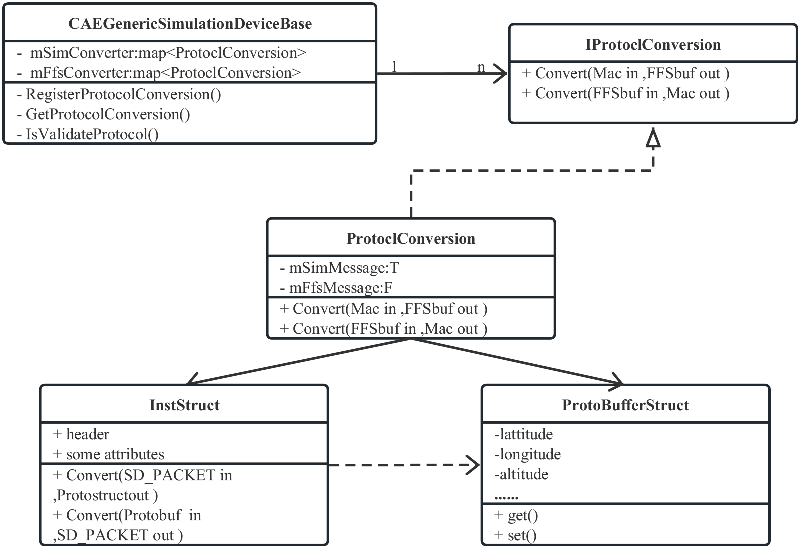
\includegraphics[width=\textwidth]{pictures/classdiagram2.pdf}
        \caption{指令转换核心类图}
        \label{module22}
    \end{center}
\end{figure}
\subsection{顺序图}
图\ref{seq2}是协议转换模块的顺序图。描述了仿真机指令与自定义指令的转换中各类的交互过程。
在系统启动后,CAEDevice的构造函数会完成所有转换器的注册,即将指令代号与指令转换器作为键值对加入map中。
在指令转换前,需要先通过指令代号到map中获取对应的转换器。
调用实例化转换器中的Convert方法时,该方法会调用到仿真机指令中的Convert实现方法。
\begin{figure}[h!]
    \begin{center}
        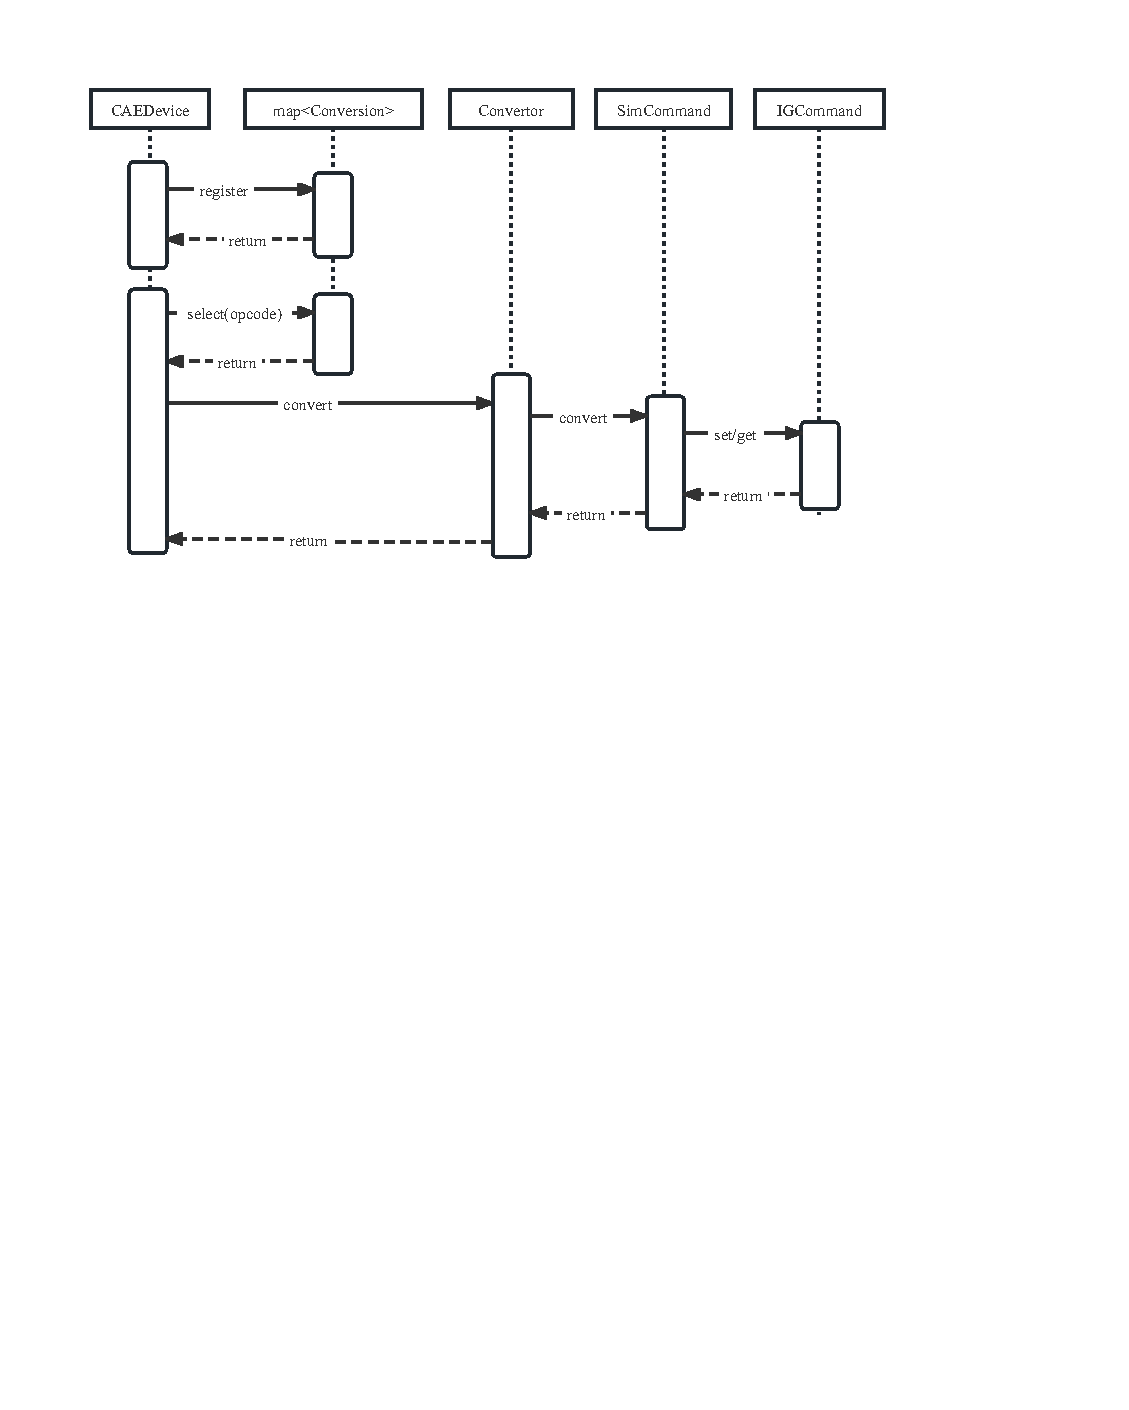
\includegraphics[width=\textwidth]{pictures/sequence2.pdf}
        \caption{指令转换顺序图}
        \label{seq2}
    \end{center}
\end{figure}
\subsection{关键代码}
指令转换模块负责仿真机指令与自定义指令间的转换。关于仿真机指令的结构前文已有详细介绍,
自定义指令的结构如图\ref{protostruct}所示。这是proto文件中定义的结构化数据,因为本文使用到二进制交换协议ProtoBuffer,发送方与接收方都必须清楚结构才能正常序列化与反序列化。
最上层的FFSFrame结构是虚拟仿真机与图像生成器交流时使用的通用结构,其头部信息中包含发送方、接收方、发送时间等。最后带有一个可重复的字段packets,代表多个自定义指令。
\par
中间的FFSPacket则表示单一的自定义指令,第一个枚举类型代表指令代号,第二个bytes类型的字段content则是已经经过序列化的该指令具体内容。接收方可以根据opcode信息实现content的反序列化。
最后则是一个自定义指令的具体案例,AircraftGcsStatus是用于更新飞机位置和姿态的自定义指令,其中含有当前帧飞机在笛卡尔坐标系中的位置以及旋转姿态。
\par
完成proto文件的编写后,就可以用对应的ProtoBuffer编译器将该文件编译成目标语言。如果编译为C++后会得到.pb.h和.pb.cc文件,分别表示自定义指令的头文件和实现文件,
其中提供了一系列的get/set函数用来修改和读取结构化数据中的数据成员。当需要将该结构化数据序列化时,类中已经提供相应的方法来把对象变成字节序列。
对想要读取数据的一方来说,也只需要使用类中的反序列化方法来将这个字节序列重新转换为结构化数据。
\begin{figure}[h!]
    \begin{center}
        \lstinputlisting[basicstyle= \zihao{-5}]{pictures/ProtoStruct.txt}
        \caption{自定义指令结构}
        \label{protostruct}
    \end{center}
\end{figure}
\par
图\ref{21convert}是一对指令转换的实现。该方法将仿真机中负责飞机位置和姿态调整的21H号指令,转换为自定义指令AircraftGcsStatus。
该对于仿真机指令中的浮点数据一般都需要进行数字表示方式的转换后才能赋值给自定义指令。该指令中比较特殊的一点是,仿真机是通过经度纬度和海拔给出的飞机位置,而图像生成器中需要使用地心地固坐标系这种笛卡尔系确定位置。
其中涉及到坐标系间的转换。而飞机的旋转是在该位置的东北天坐标系下定义,该坐标系三个轴分别是与大地水准面相切的东方,北方以及地表的法线方向。
\begin{figure}[h!]
    \begin{center}
        \lstinputlisting[basicstyle= \zihao{-5}]{pictures/21Convert.txt}
        \caption{指令转换代码}
        \label{21convert}
    \end{center}
\end{figure}
\par
由大地经度,大地纬度和海拔高度组成的LLA坐标系,是广泛应用的一个地球坐标系。
这里需要说明大地纬度的定义并不是某点同地心连线后与赤道平面的夹角,而是该点地表法线与赤道平面的夹角。如图\ref{latitude}所示由于地球是一个两级略扁的椭球体,这两种定义并不相同。
海拔高度的定义也是沿法线的方向到地表的距离。
地心地固坐标系ECEF是以地心为原点,x轴指向赤道与本初子午线的交点,y轴指向北地极,z轴由手性决定的笛卡尔坐标系。
\begin{figure}[h!]
    \begin{center}
        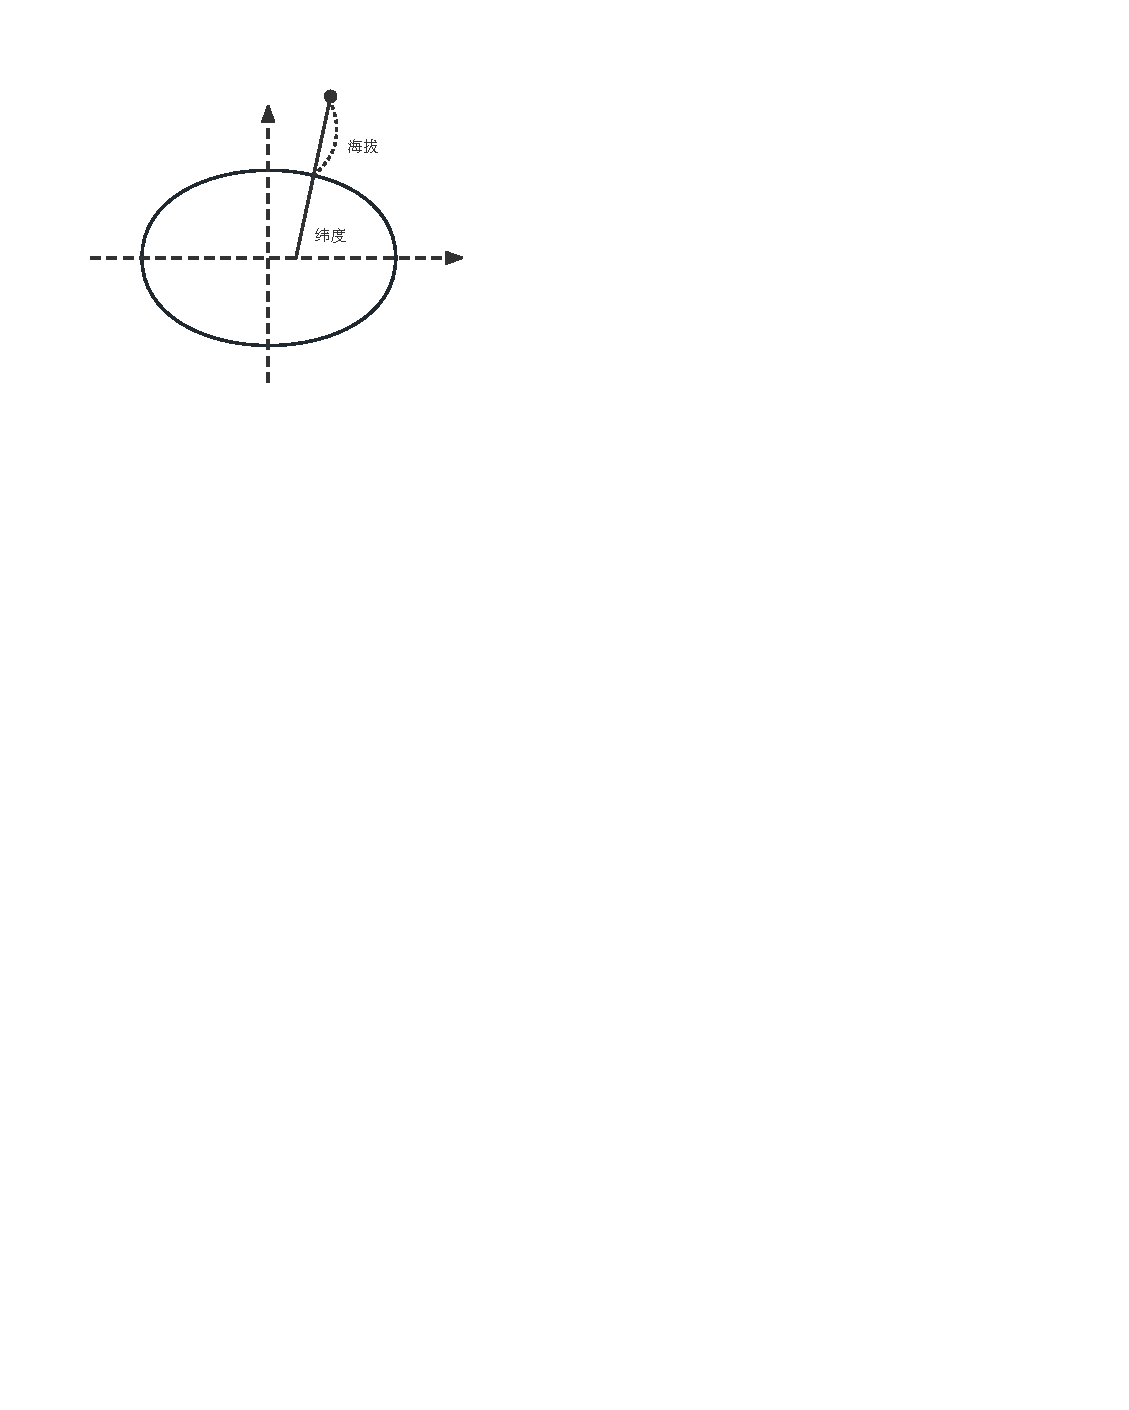
\includegraphics[width=0.5\textwidth]{pictures/latitude.pdf}
        \caption{纬度示意图}
        \label{latitude}
    \end{center}
\end{figure}
\par
图\ref{LLA2ECEF}中的代码给出了经纬度海拔坐标系LLA转换为地心地固坐标系ECEF的算法。
在两种坐标系下地球都是默认为两级略扁的规则椭球体,赤道长半轴为6378137.0米,两极短半轴为6356752.314245米,扁率为1/298.257223563。
B. R. Bowring在1985年便提出了两种坐标间的转换方法\cite{cha4}。代码中a为长半轴,b为短半轴,e为椭球的偏心率,N为椭球的曲率半径。
最后对z轴调整手性是为了配合图像生成器中使用的左手系。
$$e^2=\frac{a^2-b^2}{a^2}$$
$$N=\frac{a}{\sqrt{1-e^2sin^2(lat)}}$$
\begin{figure}[h!]
    \begin{center}
        \lstinputlisting[basicstyle= \zihao{-5}]{pictures/LLA2ECEF.txt}
        \caption{LLA转ECEF坐标算法}
        \label{LLA2ECEF}
    \end{center}
\end{figure}
\par
飞机的旋转姿态定义在东北天坐标系下,最终需要将该旋转由东北天坐标系复原到世界坐标ECEF下。
为此要得到东北天坐标系的三个坐标轴在世界坐标系中的投影。
我们可以根据经度和纬度做简单的三角函数运算得出该点法线向量normal,即ENU坐标系中的up方向。同时法线与ECEF坐标中的y轴所构成的平面一定与东方向垂直。
在三维向量下,两个不平行的向量进行叉乘可以得到垂直于该平面的一个向量。将normal与y轴单位向量(0,1,0)叉乘即可得到东方向。同理将东方向与normal叉乘,即可得到北方向。
飞机的姿态需要使用欧拉角与东北天坐标系形成的旋转矩阵相乘,才能正确得到图像生成器世界坐标系下的姿态。
\begin{eqnarray}    \label{eq}
    normal.x&=&cos(lat) * sin(lon)  \nonumber    \\
    normal.y&=&sin(lat) \nonumber    \\
    normal.z&=&-cos(lat) * cos(lon) \nonumber
\end{eqnarray}
\section{图像生成器侧数据交换模块}
图像生成器数据交换模块负责图像生成器与虚拟仿真机之间的交流。其利用Tbuspp插件使用TCP协议沟通,数据交换协议则是ProtoBuffer。
此过程中为了对自定义指令添加头部信息构建通用结构,需要对两次序列化,解封过程同样需要两次反序列化。
\subsection{流程图}
 本模块的主要执行流程如图\ref{module31}所示。当收到来自指令转换模块的自定义指令时首先将其进行一次序列化。为了保证接收方了解怎样反序列化,还需要为序列添加指令代号,相当于生成了一个虚拟仿真机与图像生成器间交流的通用指令结构。将此结构再一次序列化后可以加入到Tbuspp发送队列中进行发送。
 而当从Tbuspp的接收队列中读取了反馈信息后,需要使用通用结构第一次反序列化得到指令代号,根据指令代再使用对应自定义指令结构对剩余部分反序列化。便可以将得到的自定义指令交给指令转换模块。

 \begin{figure}[h!]
    \begin{center}
        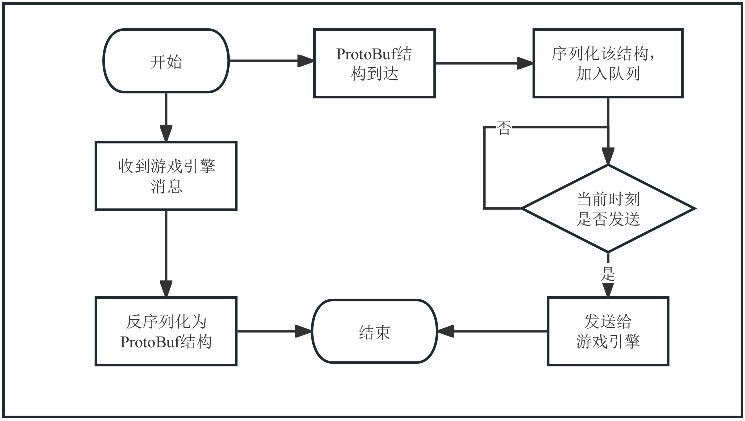
\includegraphics[width=0.8\textwidth]{pictures/flowchart3.pdf}
        \caption{图像生成器侧数据交互流程图}
        \label{module31}
    \end{center}
\end{figure}
\subsection{核心类图}

本模块的核心类图如图\ref{module32}所示。其中的核心是类ImageGeneratorContext,它表示图像生成器与虚拟仿真机的交流环境,其中主要的成员是代表信息收发进程的ImageGeneratorTaskRunnable。
该类中的mAssembler成员负责在需要发送自定义指令时为其指令添加代号等头部信息,生成通用结构FFSPacket。多个FFSPacket可以粘合为一个FFSFrame一起发送。
\par
MsgHandler则是在图像生成器侧信息接收部分的专属类。不同于虚拟仿真机接收到自定义指令后不区分类别的将其交给指令转换器,图像生成器需要根据不同的指令调用不同的逻辑执行。
比如收到控制飞行的指令后,就需要将其中的数据给到飞机实体。具体方法由实现类中的OnExecutedImpl实现。
\begin{figure}[h!]
    \begin{center}
        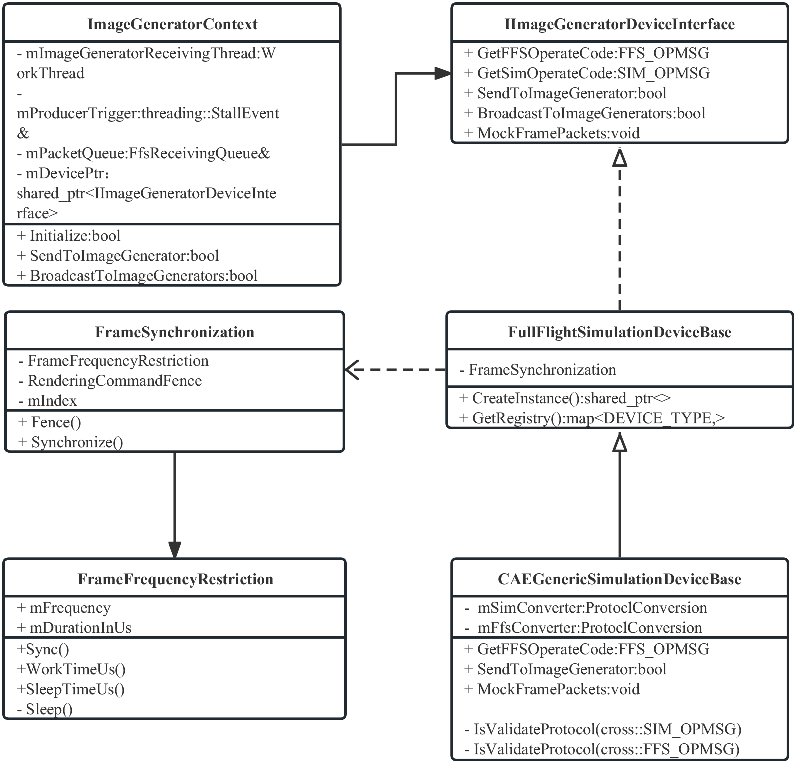
\includegraphics[width=\textwidth]{pictures/classdiagram3.pdf}
        \caption{图像生成器侧数据交互核心类图}
        \label{module32}
    \end{center}
\end{figure}
\subsection{顺序图}
图\ref{seq3}是图像生成器侧数据交换模块的顺序图。描述了虚拟仿真机与图像生成器间沟通时各类的交互过程。
在系统初始化时,IGContext会首先通过Tbuspp的配置文件初始化交流环境。需要发送信息时,交流环境会通过send方法将自定义指令交给进程实例,该进程实例会调用Assembler中的封装流程获得指令通用结构,最后调用Tbus中的发包方法完成发送。
接收数据时,进程实例会首先通过popPacket读取Tbus的接收队列,随后将信息交给Assembler类进行解封反序列化等一系列操作,虚拟仿真机中流程到这一步便结束,图像生成器中则还需要将指令分发给对应的handler进行处理。

\begin{figure}[h!]
    \begin{center}
        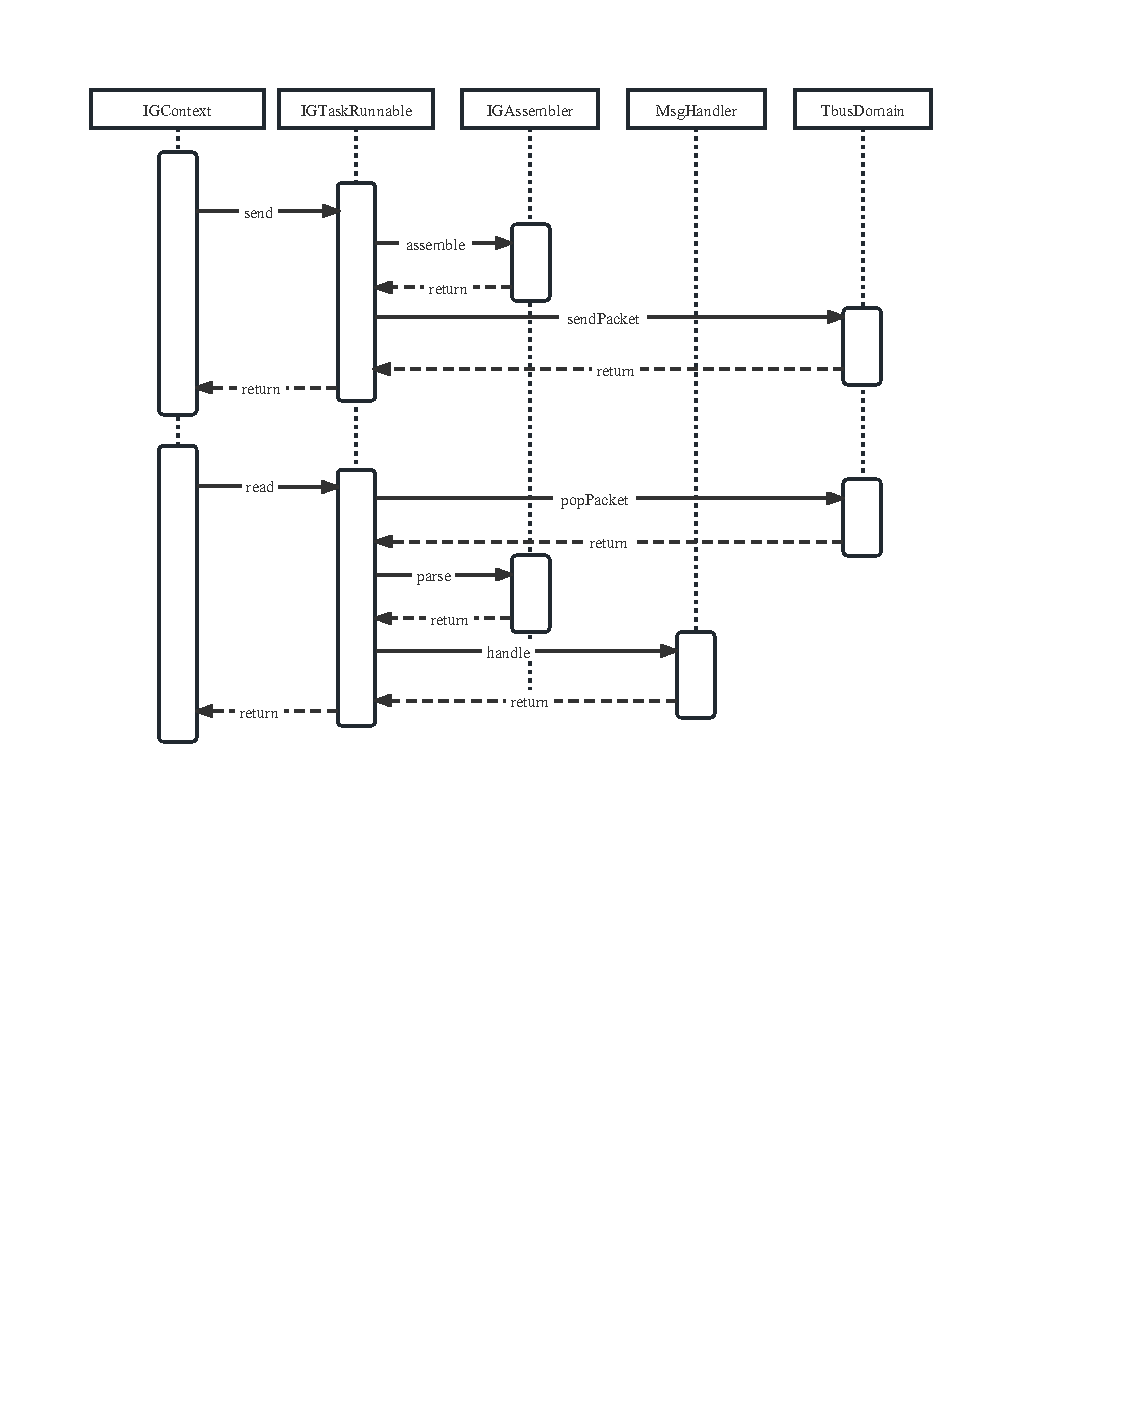
\includegraphics[width=\textwidth]{pictures/sequence3.pdf}
        \caption{图像生成器侧数据交换顺序图}
        \label{seq3}
    \end{center}
\end{figure}
\subsection{关键代码}
图\ref{IGsend}中的代码展示了将一组自定义指令封装为一个通用结构FFSFrame并发送的过程。
首先为outFFSFrame添加虚拟仿真机的版本信息version,方便对开发过程中的不同版本进行对比。
之后需要将全部的自定义指令逐一进行序列化并添加于outFFSFrame的对应字段中。全部添加完成后使用AssembleFrameHeader方法为其添加发送方、接受方、发送时间等信息再次序列化。
进入消息发送阶段,每一个Tbuspp的终端都有唯一的ID,发送前需要查找接收方的ID后通过QueuePacket方法将该序列写入对应的发送队列。
\begin{figure}[h!]
    \begin{center}
        \lstinputlisting[basicstyle= \zihao{-5}]{pictures/IGSend.txt}
        \caption{自定义指令封装代码}
        \label{IGsend}
    \end{center}
\end{figure}
\par
图\ref{tbusio}中的代码展示了Tbuspp在发送和收取信息时的一些细节。发送函数QueuePacket中,参数busid表示数据的接受方,inData是将要发送数据的指针,
inSize是该数据的长度。首先如果发送队列指针为空则说明未正确初始化。之后根据busid获得接收方实例,同时配置使用一些默认的发送控制参数param。
在写入队列时,需要保证线程安全,写入前先使用mutex为该区域加锁,随后向out\_queue中写入从inData开始长度为inSize字节的内容。
\par
接收消息时,首先定义信息缓冲区buffer,长度为1024字节,因为经最初的抓包经验可知不会存在更大的包。
通过tbuspp\_queue\_peek方法获取到消息的指针msg,和消息的长度outSize。随后将从msg开始,长度为outSize的信息拷贝到buffer完成消息读取。
最后将接收队列中的该消息移出队列。
\begin{figure}[h!]
    \begin{center}
        \lstinputlisting[basicstyle= \zihao{-5}]{pictures/TbusIO.txt}
        \caption{Tbuspp收发消息代码}
        \label{tbusio}
    \end{center}
\end{figure}
\par
虚拟仿真机与图像生成器之间通过通用指令结构进行沟通,在接收到通用结构后需要进一步解封获取自定义指令。
图\ref{IGrecv}中给出了图像生成器接收到消息后进行解封并交付使用的过程。
首先依旧是从tbuspp接收队列中读取消息,反序列化后将其中的自定义指令依次加入circular\_queue中,使用自定义指令的逻辑线程会从该队列中拿取指令。
\par
OnHandleTbusppPacket是对自定义指令进一步反序列化并交付使用的过程。当队列中存在自定义指令时,会根据指令的opCode从handlerMap中查找对应的处理者,
该处理者会调用OnExecuted方法会将指令数据给到mGameWorld中需要它的实体。
\begin{figure}[h!]
    \begin{center}
        \lstinputlisting[basicstyle= \zihao{-5}]{pictures/IGReceive.txt}
        \caption{通用结构解封代码}
        \label{IGrecv}
    \end{center}
\end{figure}


\section{本章小结}
本章在需求分析及概要设计的基础上,对系统包含的仿真机侧数据交换模块、指令转换模块和图像生成器侧数据交换模块的详细设计与实现做了阐述。
详细设计通过流程图、核心类图和顺序图说明了运行过程中各个类之间的交互逻辑,实现则是通过解读关键代码的方式进行说明。
